\section{Design Goal}\label{sec:goals}
The goal of the IDDR system is to provide full isolation between a device driver and the monolithic kernel and at the same time avoid modifications to the device driver code. The goal of the thesis is to minimize the performance penalty because of the communication between the domains. In the thesis, we explore opportunities to minimize the overhead of the communication module in the IDDR system.

\subsection*{Performance Improvement}
The IDDR system is a re-implementation of the Xen's isolated driver domain. Even though the IDDR system provides better robustness for the operating system, it deteriorates the performance. The reasons for the performance deterioration is due to the introduction of hypervisor, data copy overhead or overhead of communication between the domains. 

\paragraph{Hypervisor Layer: } The IDDR system uses Xen hypervisor as a virtualization platform. Xen hypervisor is a Type 1 hypervisor. A type 1 hypervisor runs directly on the host's hardware. It runs between the operating system and the hardware. In Xen, the hypervisor runs in ring 0, while guest OS runs in ring 1 and applications run in ring 3. For hardware access, the guest OS has to go through the hypervisor, which degrades the performance of the system

\paragraph{Copy Overhead: } For data intensive operations such as read and write, the IDDR system transfers data between the hardware and the driver domain. It also transfers the same data between the driver domain and the application domain. The extra copy from the driver domain to the application domain is also one of the reasons for the performance degradation of the system. 

\paragraph{Communication Channel Overhead: } The IDDR system runs a device driver in a separate domain called the driver domain. The application domain and the driver domain communicate with each other in order to send requests and get responses from the device driver. The communication between domains add an overhead to the system performance. Our goal is to minimize the overhead during communication between the driver domain and the application domain.

\section{Isolated Device Driver Properties}
\label{sec:properties}
This section covers the properties of the base IDDR system. As we are explore the opportunities to improve the performance of the base IDDR system, it is necessary that these properties are not compromised.

\subsection*{Strong Isolation}
One of the main properties of the IDDR system is strong isolation. The IDDR system adds an extra layer of isolation in the design which provides fault isolation between the kernel and the device driver. The strong isolation also adds the ability to manage device drivers independently, thus, increasing the availability of the system during maintenance of a device driver.

\subsection*{Compatibility and Transparency} 
The extension of existing OS structures usually results in a large number of broken applications. As a specific example, in the microkernel architecture the functional units of an OS were divided into discrete parts in order to achieve the isolation between the kernel components. As a result, the APIs visible to applications were changed~\cite{hand2005virtual}, which broke the large number of applications. In order to provide compatibility with applications, many microkernel architectures provided an emulation layer~\cite{hand2005virtual} for the OSes. The IDDR system maintains compatibility between existing device drivers and applications.

\section{System Overview}\label{overview}

Figure~\ref{fig:monolithic} presents the architectural overview of the modern operating system with a monolithic kernel and Figure~\ref{fig:base IDDR system overview} presents the architectural overview of the IDDR system.
\\[3mm]
\begin{figure}[!ht]
\centering
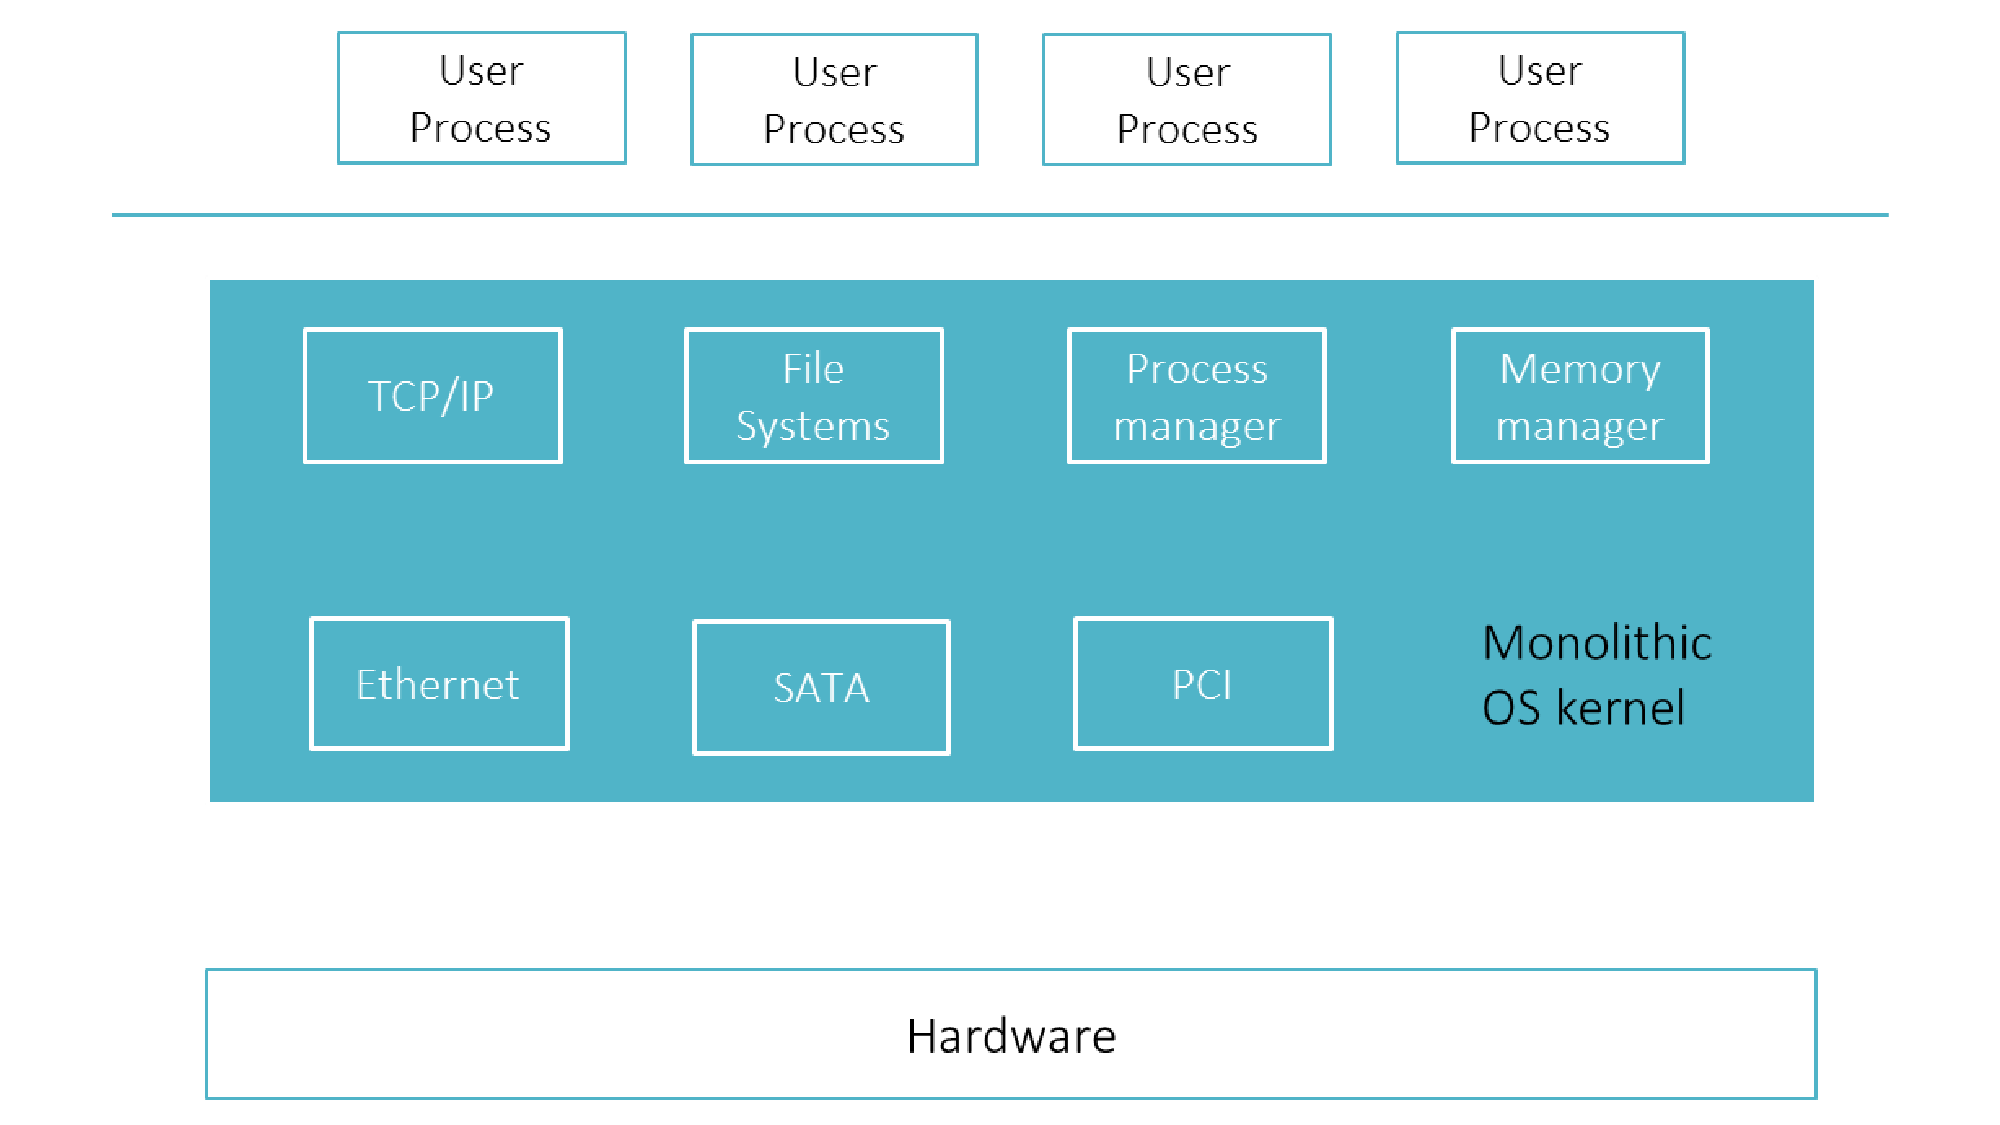
\includegraphics[scale=.5]{OSoverview}
\caption{Architectural overview of a modern OS}
\label{fig:monolithic}
\end{figure}

\begin{figure}[!ht]
\centering
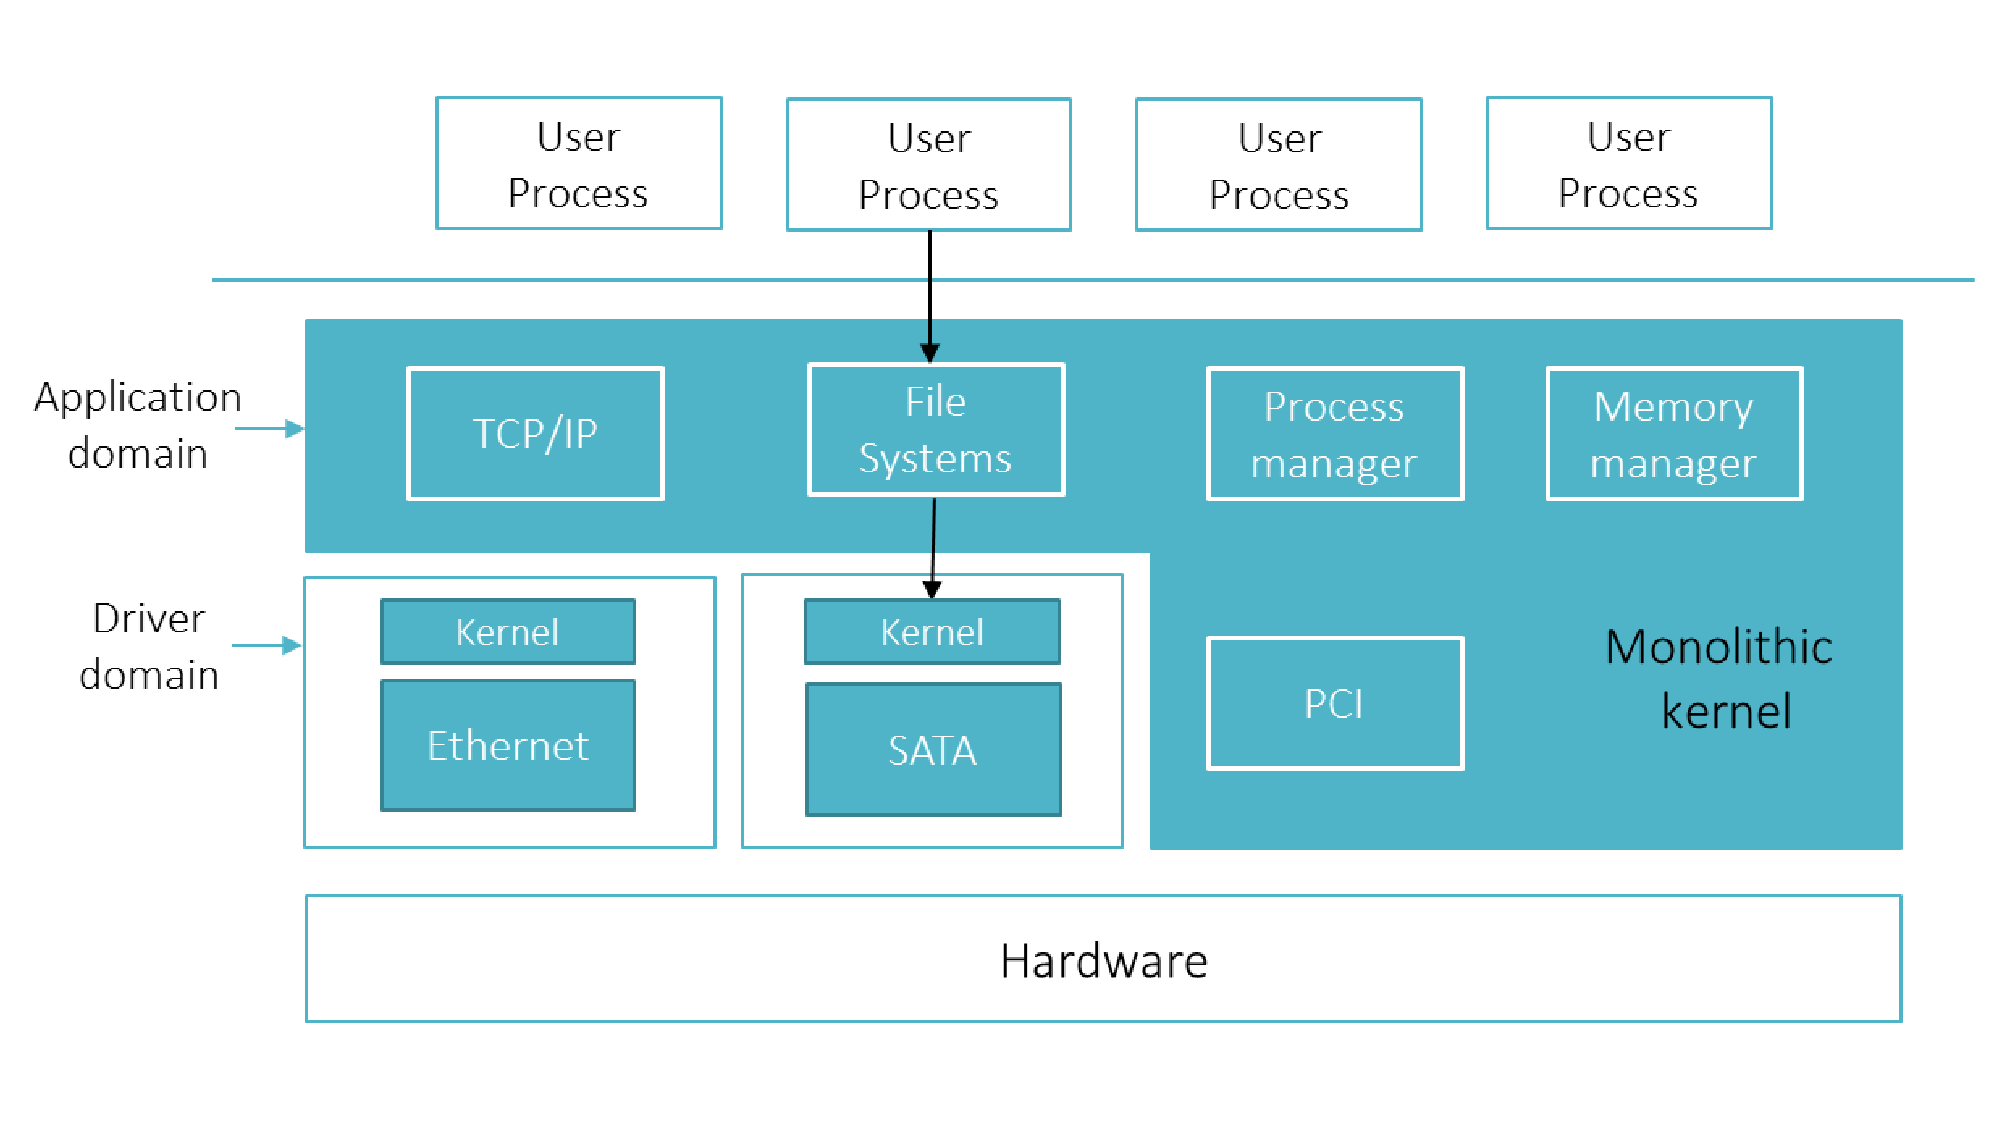
\includegraphics[scale=.5]{baseIDDRsystemoverview}
\caption{Architectural overview of the base IDDR system}
\label{fig:base IDDR system overview}
\end{figure}
The Figure~\ref{fig:base IDDR system overview} shows that the IDDR system partitions an existing kernel into multiple independent components. The user applications and Linux kernel run in a domain called the \textit{application domain}. The device driver, which needs to be isolated from the kernel, executes in the separate domain called the \textit{driver domain}. Multiple domains run on the same hardware with the help of a VMM. User applications or kernel components access the hardware through the driver domain.
\\[3mm]
As Section~\ref{sec:goals} describes, the goal of the IDDR system is to provide the isolation between the device driver and the kernel. However, a device driver is dependent on the kernel components such as a scheduler and memory management unit. In order to remove the dependency, the device driver runs closely with another instance of a kernel. Even though the dependency is removed, it is not possible to run multiple kernels over the common hardware without a virtual machine monitor. Thus, a VMM is introduced into the design to run multiple kernels on a common hardware. 

\section{System Components}\label{components}
The section describes the 3 main components of the design - frontend driver, backend driver and communication module.
\begin{figure}[!ht]
\centering
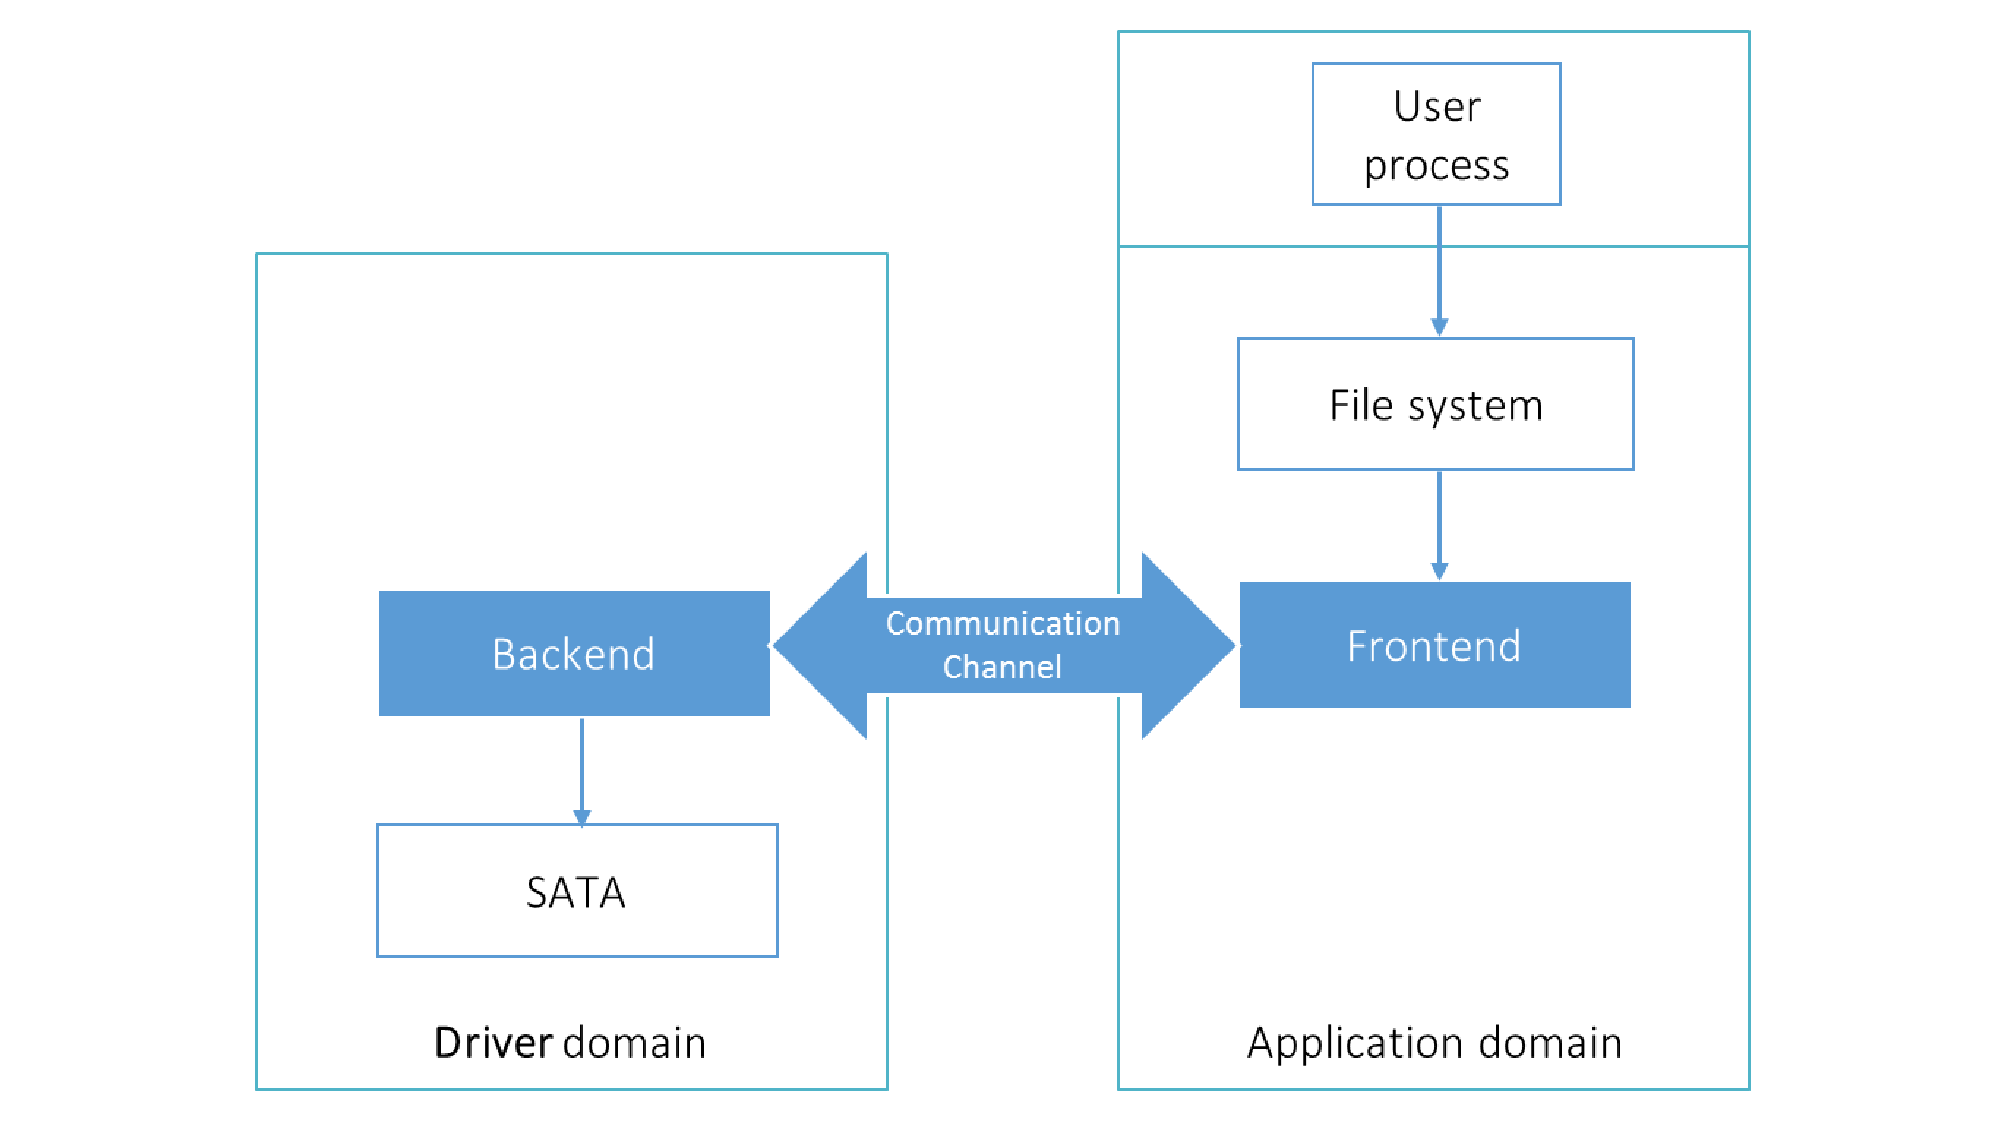
\includegraphics[scale=.5]{IDDRcomponents}
\caption{System Components}
\label{fig:Design Evo1}
\end{figure}

\subsection{Frontend Driver}
\label{subsec:frontend}
As mentioned earlier in Section~\ref{sec:properties}, transparency and compatibility are the properties of the IDDR system, which requires us to avoid any changes to the kernel, as well as the device driver. In the IDDR system, the device driver runs in the driver domain and user applications run in the application domain. Without making any changes to the kernel or applications, it is not possible for applications to send requests to the driver in the driver domain, as user applications do not know about the isolated device driver. The IDDR system runs a piece of a code called the \textit{frontend driver} in an application domain. The \textit{frontend driver} acts as a substitute for the device driver. The main functionality of the \textit{frontend driver} is to accept requests from user applications, process the requests, enqueue the requests for the driver domain and notify the driver domain. The \textit{frontend driver} reads and processes the responses received from the driver domain and ends corresponding requests.

\subsection{Backend Driver}
\label{subsec:backend}
In a Linux system, the device driver provides an interface to accept requests from user applications. However, the device driver is not capable of accepting the requests from applications running in a different domain. It cannot send responses back to the application domain without making any changes to the device driver code. In order to avoid making any changes to the device driver or the kernel, a piece of code called the \textit{backend driver} runs in the driver domain. The responsibility of the \textit{backend driver} is to accept requests from the application domain and forward them to the device driver. The \textit{backend driver} sends the responses and notifies the application domain after receiving the responses from the device driver.
\begin{figure}[!ht]
    \centering
    \begin{subfigure}[b]{0.45\textwidth}
	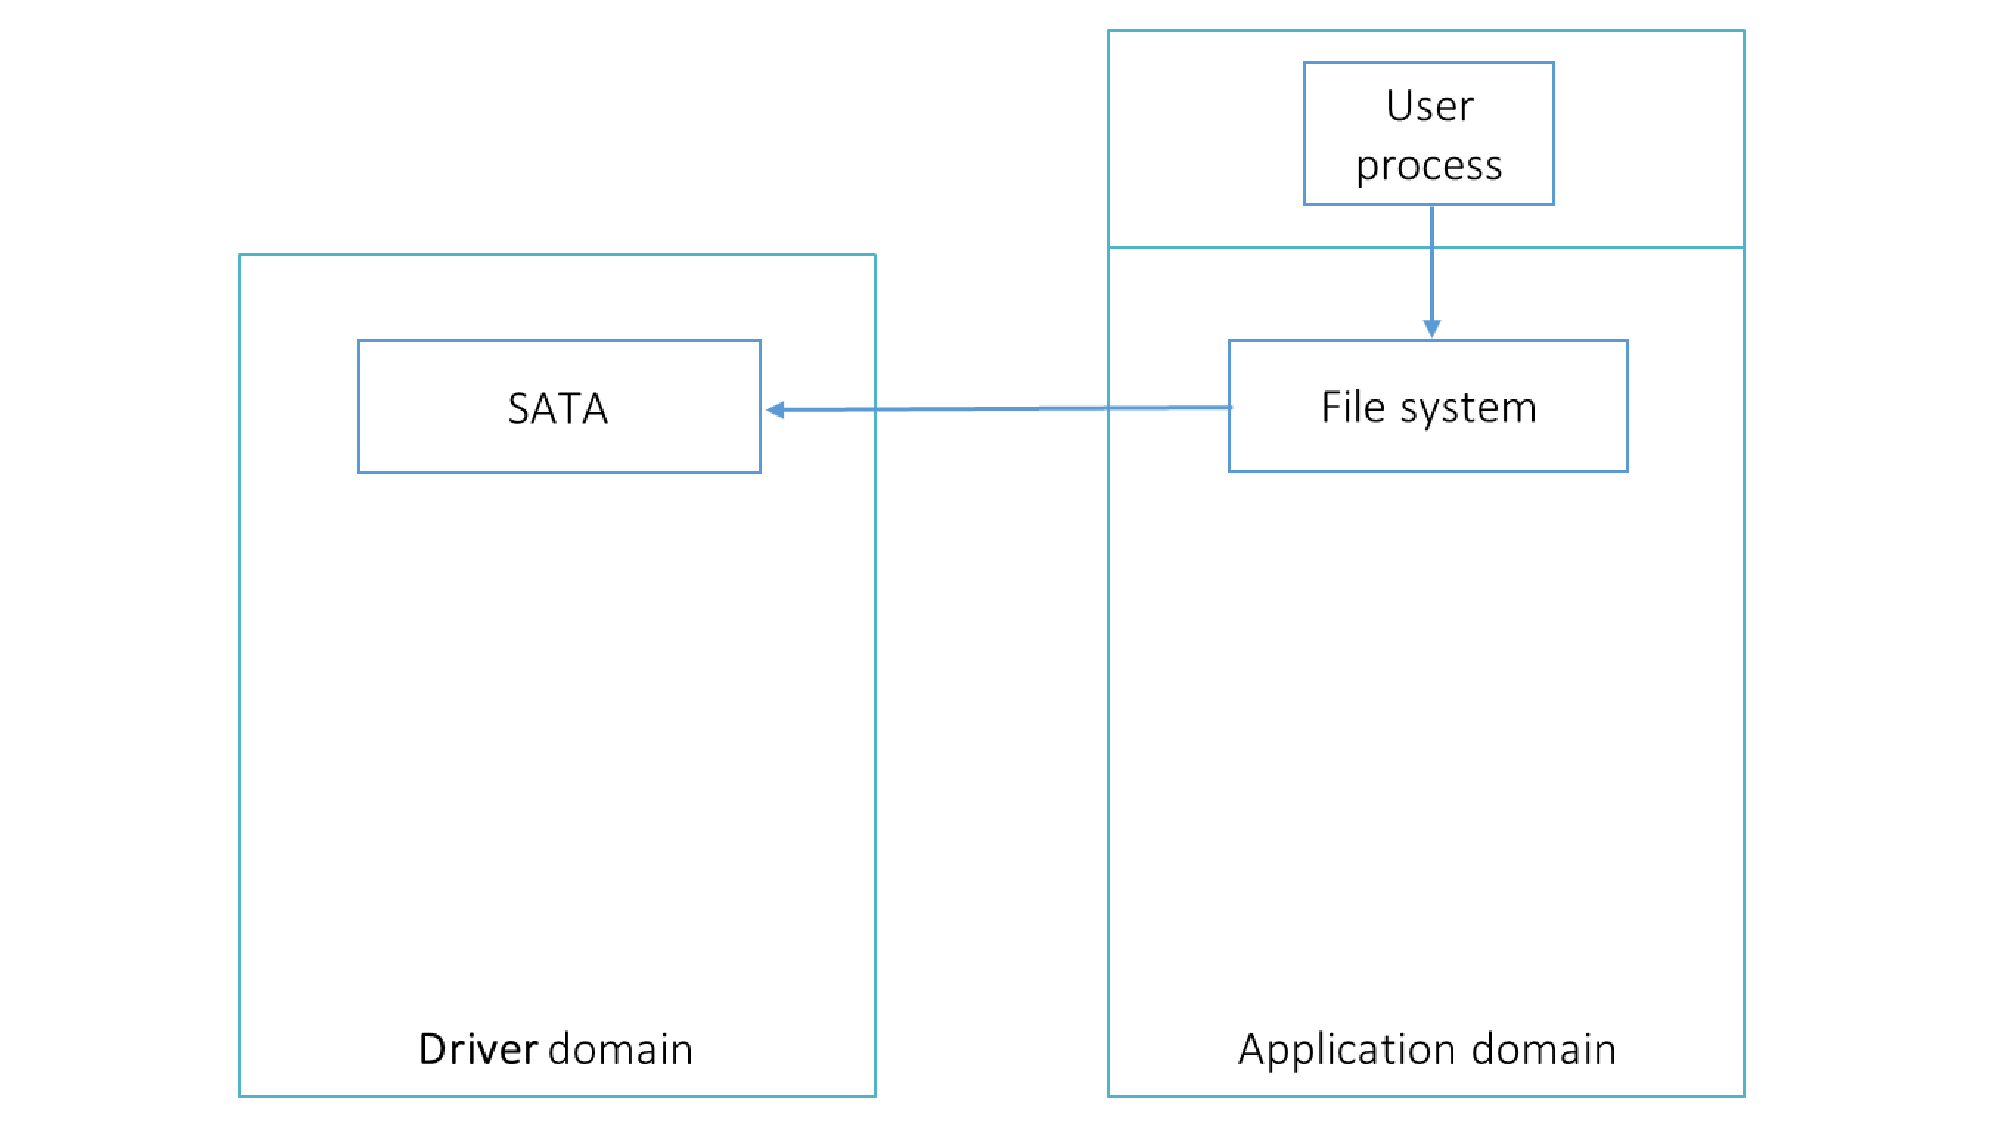
\includegraphics[scale=.25]{component1}
	\caption{Conceptual design of the driver domain}
	\label{fig:conept}
    \end{subfigure}
	\hfill
    \begin{subfigure}[b]{0.45\textwidth}
	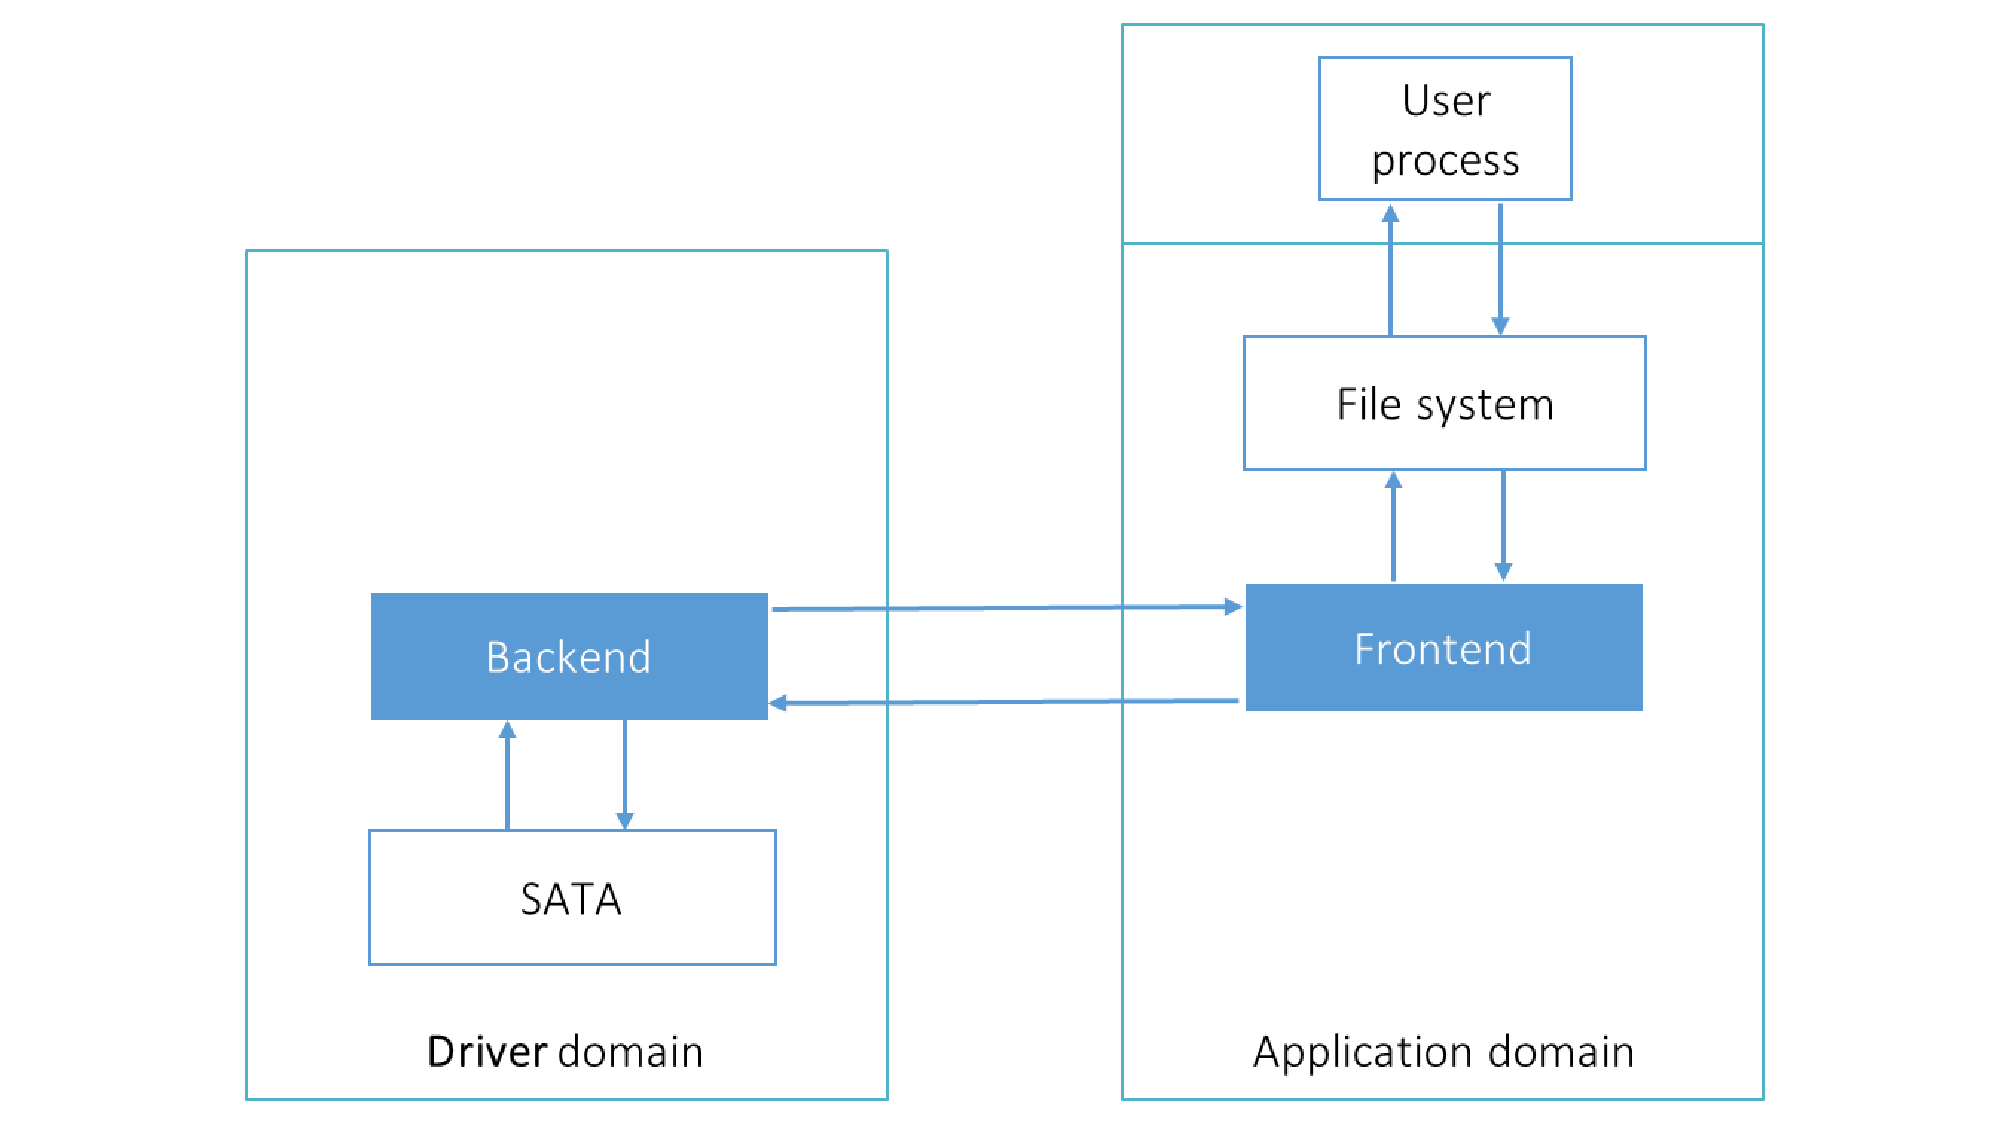
\includegraphics[scale=.25]{component2}
	\caption{Backend and frontend driver}
	\label{fig:backendfrontend}
    \end{subfigure}
    \caption{Role of the frontend and the backend driver}\label{fig:fault tolerence}
\end{figure}

\subsection{Communication Module}
\label{sub:communicationmodule}
The communication module is the communication channel between the \textit{frontend driver} and the \textit{backend driver}. Unlike the \textit{backend driver} and the \textit{frontend driver}, the communication module is not a separate physical entity or a kernel module. It exists in the \textit{frontend driver} and the \textit{backend driver}. The communication channel is logically divided into three parts. 
\begin{enumerate} 
\item The responsibility of the first part is to share the requests and responses between the driver domain and the application domain.
\item The responsibility of the second part is to share the data of read/write requests/responses.
\item The responsibility of the third part is to notify the domain upon the occurrence of a particular event. 
\end{enumerate}

Figure~\ref{fig:communication} illustrates the role of the communication model. 
\begin{figure}[!ht]
\centering
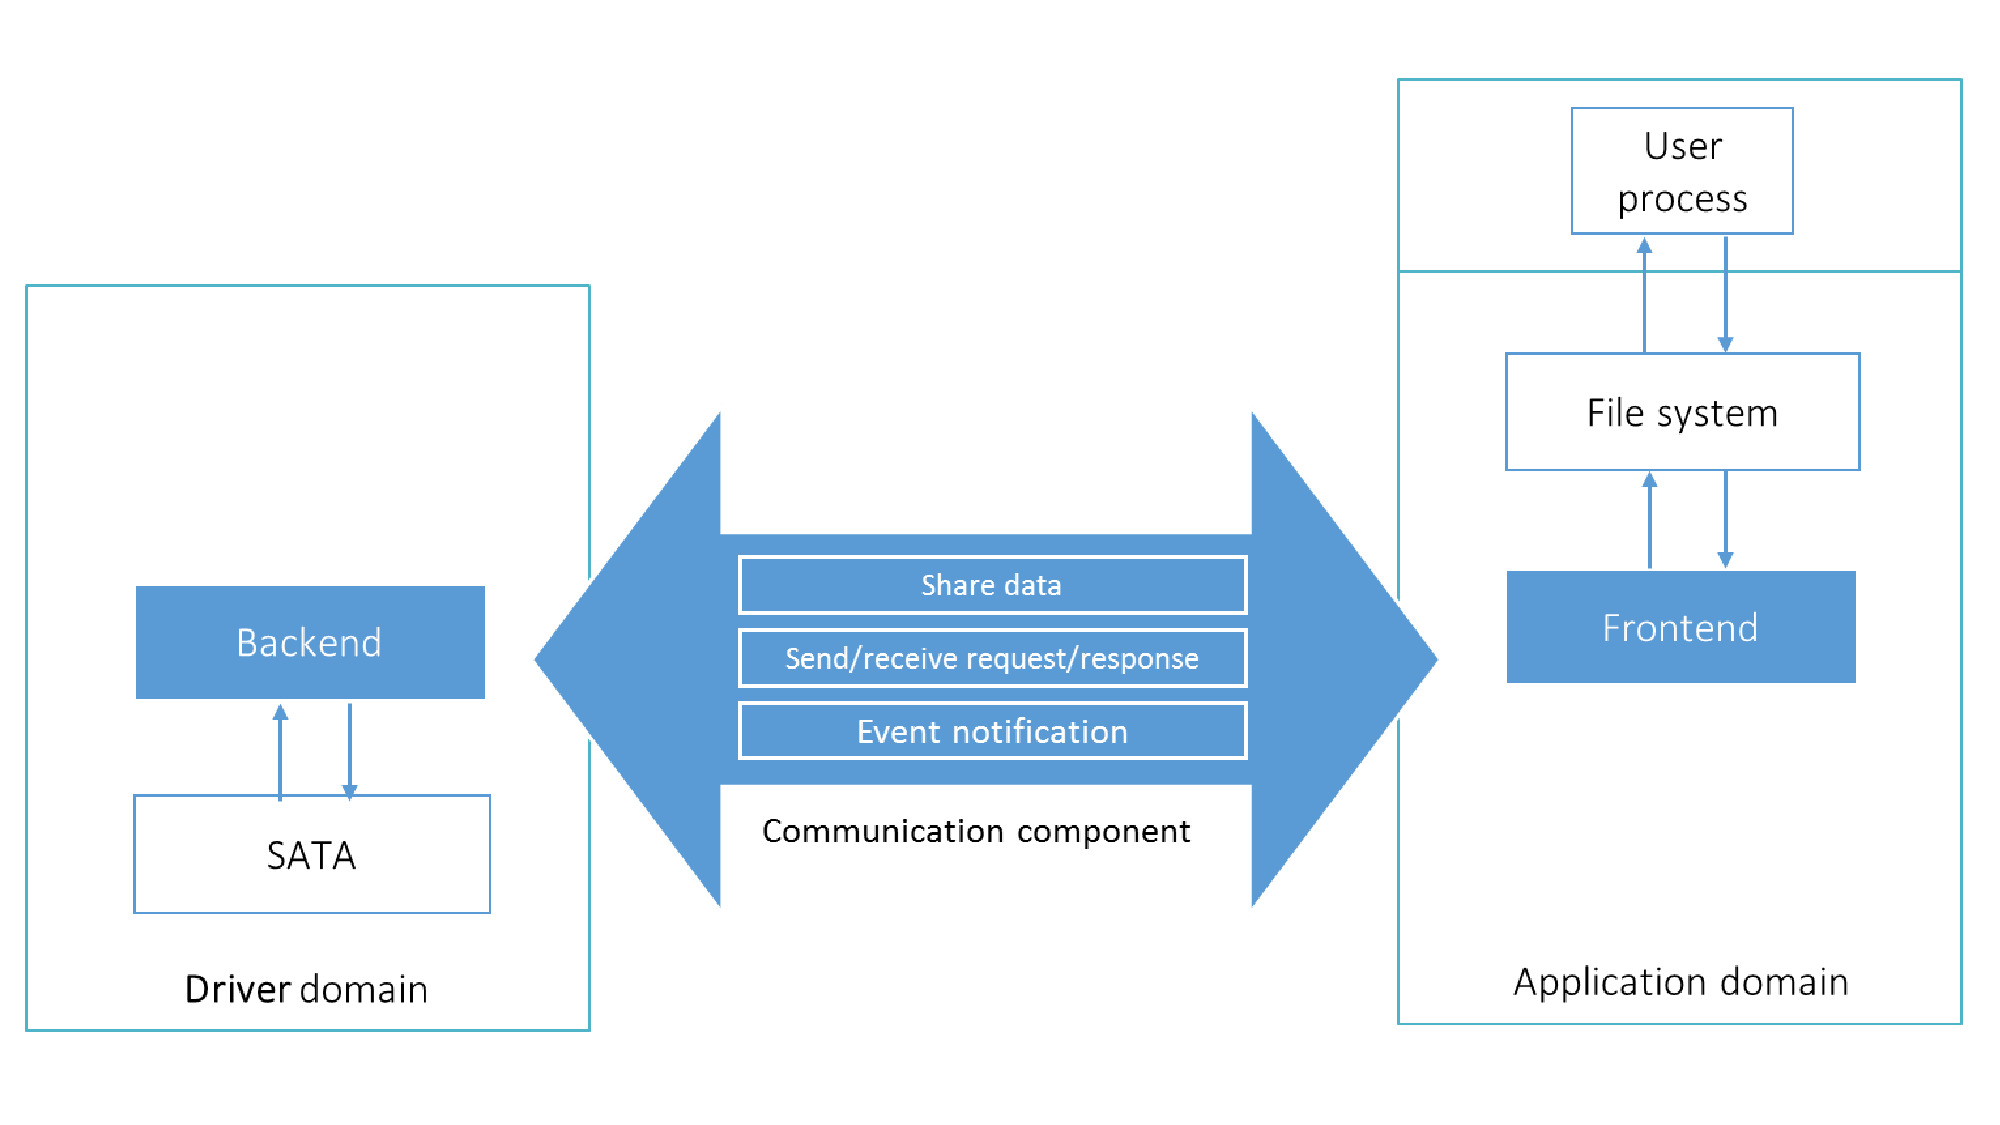
\includegraphics[scale=.5]{communicationmodule}
\caption{Communication Module}
\label{fig:communication}
\end{figure}

\section{System Design}\label{design}

The following section describes the design of the base IDDR system and the new IDDR system. 

\subsection{Communication Module}

\paragraph{Base IDDR System Design:}
\label{par:base IDDR communication}
In the base IDDR system, the frontend driver submits requests to the communication module. The communication module copies data of the write requests in a shared memory. The communication module is responsible for the allocation and de-allocation of the shared memory. Once the sufficient number of requests are submitted by the frontend driver, the communication channel shares the requests with the backend driver. It notifies the backend driver that requests are available in a shared request queue.

\paragraph{Spinlock Based IDDR System:}
\label{par:spin IDDR communication}
As Section~\ref{par:base IDDR communication} describes, in the base IDDR system, the communication module notifies the backend driver about the avaiability of reqesuts in the shared queue. A software interrupt is sent to the domain as a notification. Each software interrupt which is sent for the availability of requests, causes the hypervisor to schedule the driver domain. Similarly, a software interrupt, which notifies the availability of responses, causes the hypervisor to schedule the application domain. The scheduling of the driver domain and the application domain might result in a context swtich. 
\\[3mm]
In order to avoid the context switch, we run an intermediate thread in the frontend driver and an intermediate thread in the backend driver. Both these threads spin for the availability of requests and responses in the shared queue. The intermediate threads delegate the responsibility of the notifications from the communication module to the frontend driver and backend driver. 

\subsection{Frontend Driver}
\paragraph{Base IDDR System Design:}
In the IDDR system, the frontend driver provides an interface to accept requests from a user application on behalf of the device driver. As explained in Section~\ref{subsec:request queue}, each block device driver has a separate request queue to accept requests from a user application. Similar to the block device drivers, the frontend driver also creates an individualized request queue for each device to accept requests from a user application. If sufficient requests are received, the frontend driver flushes the requests to the communication channel. The frontend driver receives a software interrupt upon availability of responses in the shared queue. The frontend driver handles the software interrupt by reading data from the shared memory and ending the request in case of a read operation. Otherwise it ends the request without accessing the shared memory.

\paragraph{New IDDR System Design:}
As explained in Section~\ref{par:spin IDDR communication}, we introduce an intermediate thread to read responses from the shared queue. The intermediate thread spins for responses. Upon availability of a response, the thread reads the response and ends the corresponding request. If the corresponding request is a read request, then the thread reads the shared data too. However, there still exists an intra-domain context switch between the frontend driver's main thread and the intermediate thread. The main thread is responsible for reading the requests from the frontend driver request queue, and flushing them to the communication channel. The main thread context switches to the intermediate thread, which spins for the responses. 
\\[3mm]
To avoid the intra-domain context switch, we introduce a spinlock in the frontend driver. In the frontend driver, the main thread spins for responses for a short time. If a response is available, then similar to intermediate thread, the main thread reads shared data and the response and ends the corresponding request. However, in case of unavailability of a response, the main thread proceeds to read the new requests from the frontend driver request queue and the intermediate thread checks for the responses.  

\subsection{Backend Driver}
\paragraph{Base IDDR System Design:}
In the base IDDR system, the backend driver receives a software interrupt from the frontend driver. In the software interrupt handler, the backend driver forwards requests to the device driver. Upon completion of requests, the backend driver reads responses and puts them in the shared queue. It also copies read operation data to the shared memory. 

\paragraph{New IDDR system Design:}
As explained in Section~\ref{par:spin IDDR communication}, we introduce an intermediate thread to read requests from the shared memory. The intermediate thread spins for requests and upon availability of a request, it forwards the request to the device driver for execution. The backend driver reads the response from the device driver and shares it in the shared queue.
\begin{figure}[!ht]
\centering
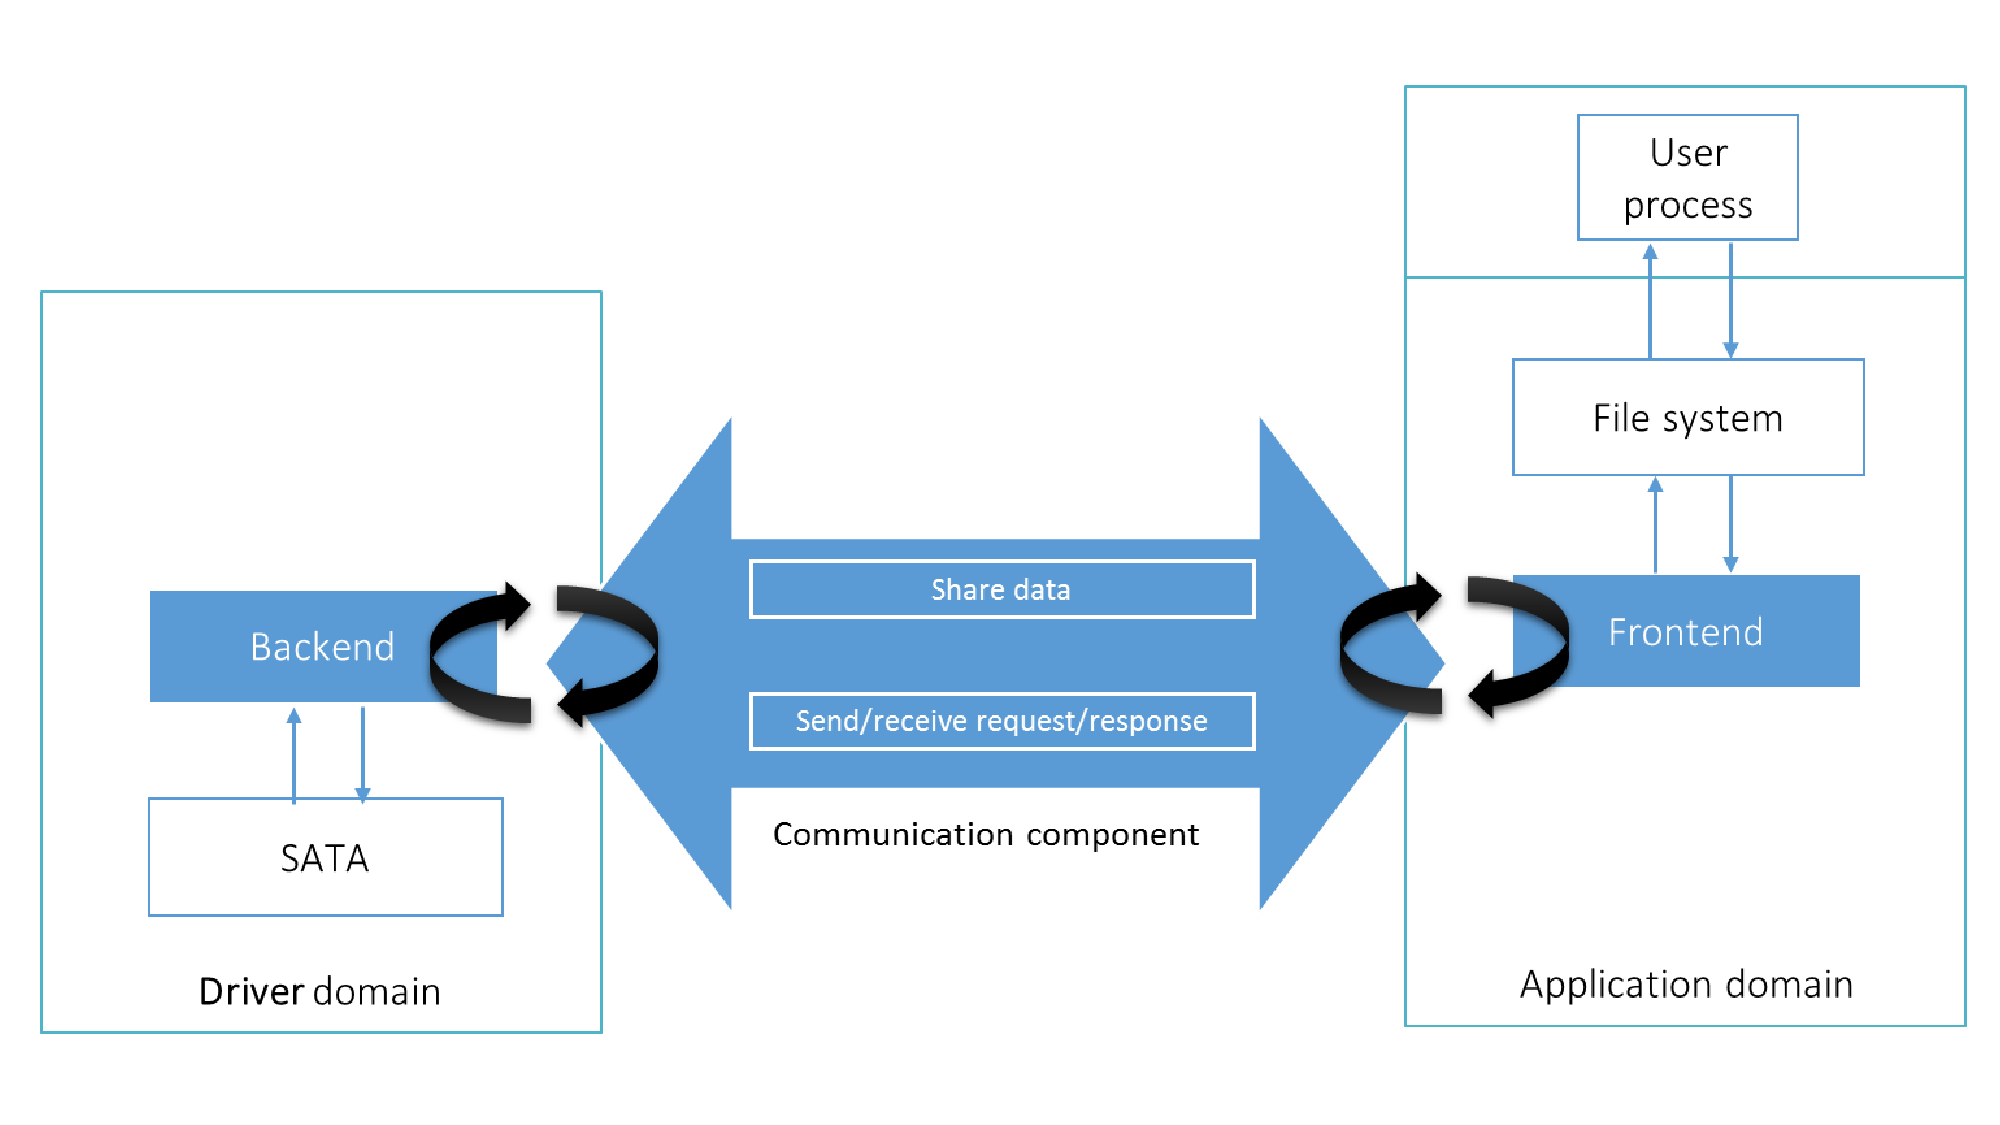
\includegraphics[scale=.5]{IDDRdesign}
\caption{Spinlock based new IDDR system}
\label{fig:new IDDR system}
\end{figure}

% \section{fault tolerance}
% Figure~\ref{fig:driver crash} and Figure~\ref{fig:high avail} explains the effects of a malicious activity occurring in the device driver isolated from the Linux kernel. When a device driver running in a driver domain hits a bug, it crashes the kernel of the driver domain and hence the driver domain itself. In addition, applications expecting a response from the driver domain might hang or crash waiting for the response. But due to the address space separation of the application domain and the driver domain, the application domain will remain intact.   
% \begin{figure}[!ht]
%     \centering
%     \begin{subfigure}[b]{0.45\textwidth}
% 	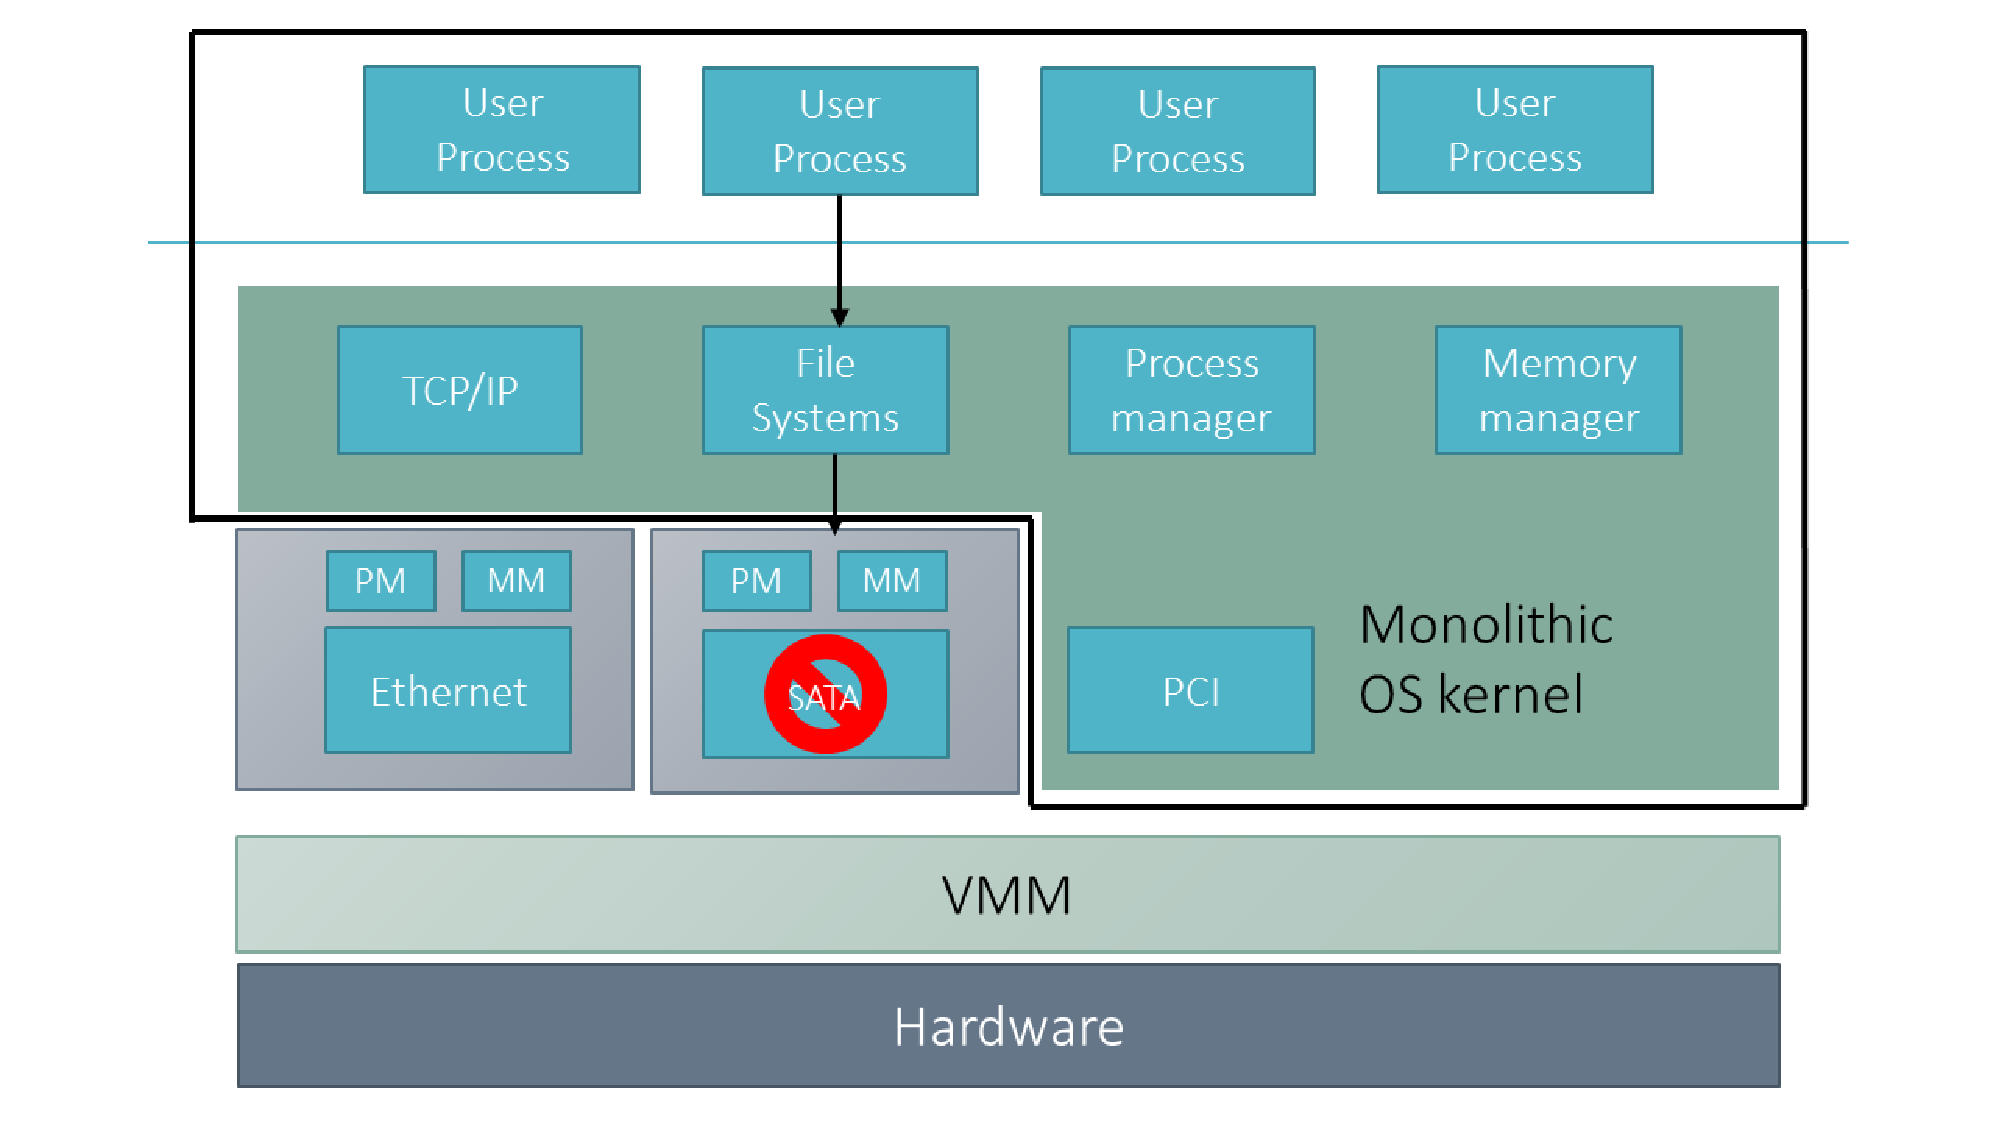
\includegraphics[scale=.25]{IDDRcrash1}
% 	\caption{Device driver crash}
% 	\label{fig:driver crash}
%     \end{subfigure}
% 	\hfill
%     \begin{subfigure}[b]{0.45\textwidth}
% 	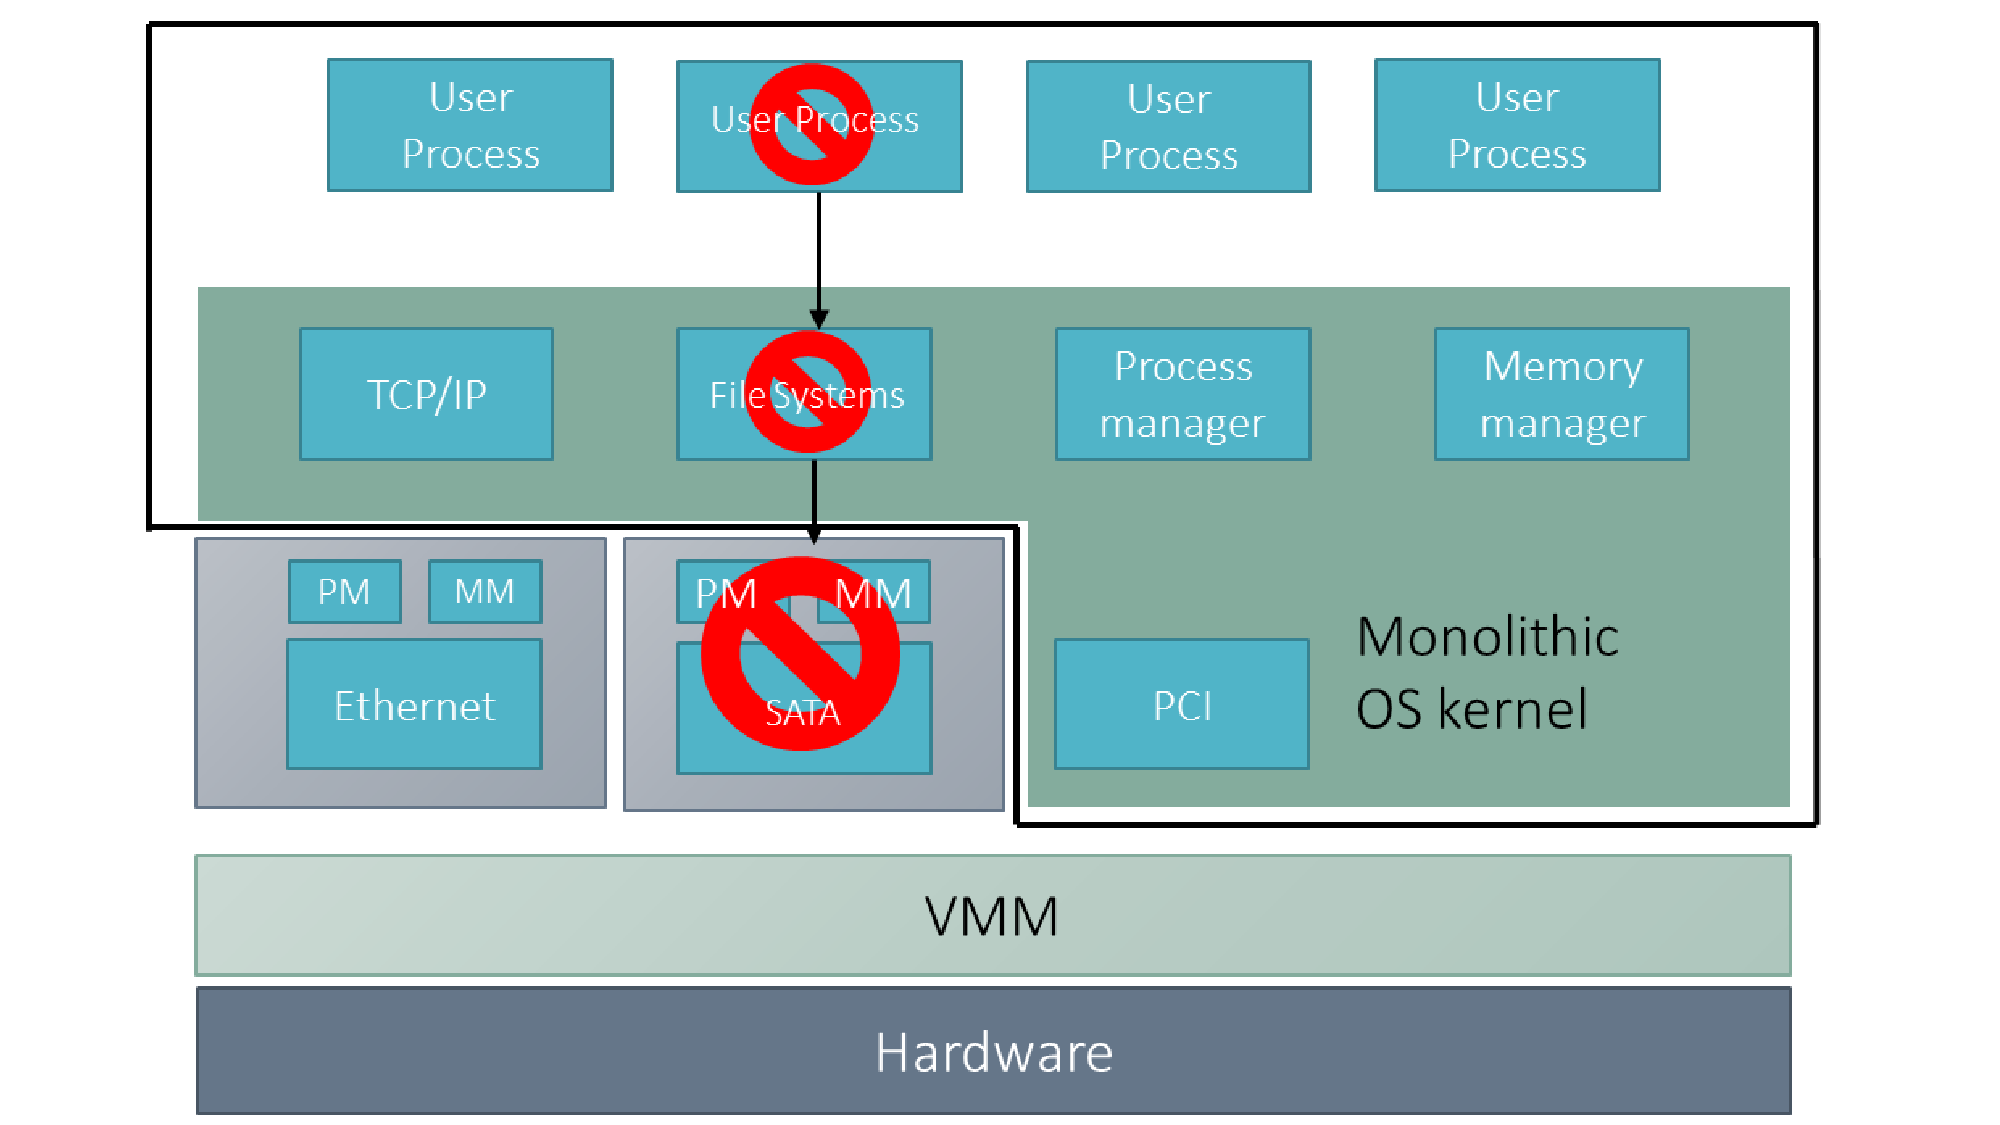
\includegraphics[scale=.25]{IDDRcrash2}
% 	\caption{Intact system}
% 	\label{fig:high avail}
%     \end{subfigure}
%     \caption{Fault tolerence}\label{fig:fault tolerence}
% \end{figure}
    
\ifbool{toShowBibliography}{\bibliography{references}}{}
